\documentclass[11pt,a4paper]{article}

% -----------------------------------------------------
%	Use packages.
% -----------------------------------------------------
\usepackage[english]{babel}
\usepackage[utf8]{inputenc}
\usepackage{csquotes}
\usepackage[left=2.5cm,right=3cm,top=3cm,bottom=3cm]{geometry}
\usepackage{subfiles}
\usepackage{helvet}
\usepackage{rotating}
\usepackage{pdflscape}
\usepackage{typearea}
\usepackage{graphicx}
\usepackage{listings}
\usepackage{pgfplots}
\usepackage{xcolor}
\usepackage{multirow}
\usepackage{mips}
\usepackage{titling}
\usepackage[automark]{scrlayer-scrpage}
\usepackage{blindtext} % Used to generate blindtext.
\usepackage{mathptmx}	% Used for Times New Roman.
\usepackage{bibgerm}
\usepackage[backend=bibtex,style=numeric]{biblatex}  %backend=biber is 'better'  
% backend = {biber, bibtex}
\usepackage{pgf}
\usepackage{tikz}
\usetikzlibrary{calc,arrows}
\usetikzlibrary{arrows,automata,positioning}
\usepackage{hyperref}

\pagestyle{scrheadings}
\pagestyle{empty}
\pagestyle{plain}


\ifoot{Hamburg University of Technology}
% -----------------------------------------------------
%	Define attributes.
% -----------------------------------------------------
\title{Advanced System-on-Chip Design}
\author{author}

\definecolor{mycolor}{RGB}{0,65,128}

\definecolor{dkgreen}{rgb}{0,0.6,0}
\definecolor{gray}{rgb}{0.5,0.5,0.5}
\definecolor{mauve}{rgb}{0.58,0,0.82}

\definecolor{myOrange}{RGB}{209,234,254}



\lstset{ %
  language=[mips]Assembler,       % the language of the code
  basicstyle=\footnotesize,       % the size of the fonts that are used for the code
  numbers=left,                   % where to put the line-numbers
  numberstyle=\tiny\color{gray},  % the style that is used for the line-numbers
  stepnumber=1,                   % the step between two line-numbers. If it's 1, each line 
                                  % will be numbered
  numbersep=5pt,                  % how far the line-numbers are from the code
  backgroundcolor=\color{white},  % choose the background color. You must add \usepackage{color}
  showspaces=false,               % show spaces adding particular underscores
  showstringspaces=false,         % underline spaces within strings
  showtabs=false,                 % show tabs within strings adding particular underscores
  frame=single,                   % adds a frame around the code
  rulecolor=\color{black},        % if not set, the frame-color may be changed on line-breaks within not-black text (e.g. commens (green here))
  tabsize=4,                      % sets default tabsize to 2 spaces
  captionpos=b,                   % sets the caption-position to bottom
  breaklines=true,                % sets automatic line breaking
  breakatwhitespace=false,        % sets if automatic breaks should only happen at whitespace
  title=\lstname,                 % show the filename of files included with \lstinputlisting;
                                  % also try caption instead of title
  keywordstyle=\color{blue},          % keyword style
  commentstyle=\color{dkgreen},       % comment style
  stringstyle=\color{mauve},         % string literal style
  escapeinside={\%*}{*)},            % if you want to add a comment within your code
  morekeywords={*,...}               % if you want to add more keywords to the set
}


\newcommand{\cacheResultFigure}[3]{
\begin{figure}
	\centering
	\includegraphics[scale=.8]{#1}
	\caption{#2}
	\label{#3}
\end{figure}
}

\newcommand{\cacheTable}[3]{
\begin{table}
\caption{#1}
\label{#2}
\begin{tabular}{lllll}
\hline %\toprule
\multirow{2}{*}{\textbf{Placement (Policy)}}& \multirow{2}{2cm}{\textbf{Block Size} \ \textbf{(Words)}}& \multirow{2}{2cm}{\textbf{Cache Hit Count}}&\multirow{2}{2cm}{\textbf{Cache Miss Count}}&\multirow{2}{2cm}{\textbf{Cache Hit Rate}} \\ & & & &  \\
\hline %\midrule
#3
\hline %\bottomrule
\end{tabular} 
\end{table}
}

\newcommand{\rowTableTestCases}[3]{\textcolor{blue}{#1} & \textcolor{blue}{#2} \\
\multicolumn{2}{l}{\parbox{15cm}{#3 \newline}} \\
\hline}




% !TEX root = fce.tex
% -----------------------------------------------------------------
% Filename  :	task4.tex
% Author    :	Carsten Hoppe
% Date		:	12. March 2017
% Reference	:	http://vhdltolatex.mamikon.net/
% -----------------------------------------------------------------

\makeatletter
\pgfdeclareshape{circuit}{
  \savedanchor\northeast{
    \pgfmathsetlength\pgf@x{\pgfshapeminwidth}
    \pgfmathsetlength\pgf@y{\pgfshapeminheight}
    \pgf@x=0.5\pgf@x
    \pgf@y=0.5\pgf@y}
  \savedanchor\southwest{
    \pgfmathsetlength\pgf@x{\pgfshapeminwidth}
    \pgfmathsetlength\pgf@y{\pgfshapeminheight}
    \pgf@x=-0.5\pgf@x
    \pgf@y=-2.65\pgf@y}
  \inheritanchorborder[from=rectangle]
  \anchor{center}{\pgfpointorigin}
  \anchor{north}{\northeast \pgf@x=0pt}
  \anchor{east}{\northeast \pgf@y=0pt}
  \anchor{south}{\southwest \pgf@x=0pt}
  \anchor{west}{\southwest \pgf@y=0pt}
  \anchor{north east}{\northeast}
  \anchor{north west}{\northeast \pgf@x=-\pgf@x}
  \anchor{south west}{\southwest}
  \anchor{south east}{\southwest \pgf@x=-\pgf@x}
  \anchor{text}{
    \pgfpointorigin
    \advance\pgf@x by -.5\wd\pgfnodeparttextbox
    \advance\pgf@y by -11.7375\ht\pgfnodeparttextbox
    \advance\pgf@y by +.5\dp\pgfnodeparttextbox}
\anchor{ina}{
  \pgf@process{\northeast}
  \pgf@x=-1\pgf@x
  \pgf@y=0.5\pgf@y}
\anchor{inb}{
  \pgf@process{\northeast}
  \pgf@x=-1\pgf@x
  \pgf@y=0.09999999999999998\pgf@y}
\anchor{inc}{
  \pgf@process{\northeast}
  \pgf@x=-1\pgf@x
  \pgf@y=-0.6000000000000001\pgf@y}
\anchor{ioa}{
  \pgf@process{\northeast}
  \pgf@y=0.5\pgf@y}
\anchor{ind}{
  \pgf@process{\northeast}
  \pgf@x=-1\pgf@x
  \pgf@y=-1.3\pgf@y}
\anchor{iob}{
  \pgf@process{\northeast}
  \pgf@y=-0.2\pgf@y}
\anchor{ine}{
  \pgf@process{\northeast}
  \pgf@x=-1\pgf@x
  \pgf@y=-2\pgf@y}
\anchor{inf}{
  \pgf@process{\northeast}
  \pgf@x=-1\pgf@x
  \pgf@y=-2.4\pgf@y}
\anchor{ing}{
  \pgf@process{\northeast}
  \pgf@x=-1\pgf@x
  \pgf@y=-2.8\pgf@y}
\anchor{inh}{
  \pgf@process{\northeast}
  \pgf@x=-1\pgf@x
  \pgf@y=-3.2\pgf@y}
\anchor{ini}{
  \pgf@process{\northeast}
  \pgf@x=-1\pgf@x
  \pgf@y=-3.6\pgf@y}
\anchor{inj}{
  \pgf@process{\northeast}
  \pgf@x=-1\pgf@x
  \pgf@y=-4\pgf@y}
\anchor{outa}{
  \pgf@process{\northeast}
  \pgf@y=-0.9000000000000001\pgf@y}
\anchor{ioc}{
  \pgf@process{\northeast}
  \pgf@y=-1.3\pgf@y}
\anchor{ink}{
  \pgf@process{\northeast}
  \pgf@x=-1\pgf@x
  \pgf@y=-4.699999999999999\pgf@y}
\anchor{inl}{
  \pgf@process{\northeast}
  \pgf@x=-1\pgf@x
  \pgf@y=-5.1\pgf@y}
\backgroundpath{
  \pgfpathrectanglecorners{\southwest}{\northeast}
  \begingroup
    \tikzset{labels}
    \tikz@textfont
  \endgroup}}
\tikzset{add font/.code={\expandafter\def\expandafter\tikz@textfont\expandafter{\tikz@textfont#1}}}
\tikzset{labels/.style={font=\sffamily\scriptsize}}
\tikzset{every circuit node/.style={draw,minimum width=5cm,minimum height=2.5cm,very thick,inner sep=1mm,outer sep=0pt,cap=round,add font=\sffamily\bfseries}}
\makeatother


% -----------------------------------------------------
%	Add bibliography resources.
% -----------------------------------------------------
%\addbibresource{references.bib}

% =====================================================
\begin{document}

% Include the titelpage.
% !TEX root = fce.tex
% -----------------------------------------------------------------
% Filename  :	titlepage.tex
% Date		:	24/01/2017
% -----------------------------------------------------------------
\begin{titlepage}
	\centering
	
\includegraphics[width=0.30\textwidth]{pictures/office_rgb_en.png}\par\vspace{1cm}
	{\scshape\LARGE Hamburg University of Technology \par}
	\vspace{1cm}
	{\scshape\Large Problem-based Learning\par}
	\vspace{1.5cm}
	{\huge\bfseries \thetitle\par}
	\vspace{1cm}
	{\Large\itshape {Carsten Hoppe} \\\href{mailto:carsten.hoppe@tuhh.de}{carsten.hoppe@tuhh.de}\par}
	\vspace{0.5cm}
	{\Large\itshape Hendrik Meyer zum Felde\\\href{mailto:hendrik.meyer@tuhh.de}{hendrik.meyer@tuhh.de}\par}
	\vspace{.5cm}
	{\Large\itshape Leonard Püttjer \\\href{mailto:leonard.puettjer@tuhh.de}{leonard.puettjer@tuhh.de}\par}
	
	\vfill	% vertikaler Zwischenraum
	Documentation	\\Advanced System on Chip \par
	
	\vfill	% vertikaler Zwischenraum
	Tutor\par
	Dipl.-Ing. Wolfgang \textsc{Brandt}

	\vfill

% Bottom of the page
	{\large \today\par}
\end{titlepage}




% Table of contents, list of figures, list of tables.
\tableofcontents
\newpage
\listoffigures
\newpage
\listoftables
\newpage
\lstlistoflistings

% -----------------------------------------------------
% Introduction.
% -----------------------------------------------------
\newpage
\section{Introduction}
% !TEX root = fce.tex
% -----------------------------------------------------------------
% Filename  :	introduction.tex
% Author    :	Leonard Püttjer
% Date		:	13. April 2017
% -----------------------------------------------------------------

This document describes a student project in the winter term 2016/2017 at the Hamburg University of Technology (TUHH). The task of the project was to extend and improve the functionality of a comparatively simple CPU, a 16-bit MIPS processing unit. For the development of our code we used the Sigasi-plugin for the Eclipse-editor. The VHDL code was compiled using GHDL and MARS and then simulated, visualized and debugged using GTKWave. We developed our source code on the three different operating systems:
\begin{itemize}
\item Windows 10 - 64 bit
\item Ubuntu 14 - 64 bit
\item macOS 10.12.4 - 64 bit
\end{itemize}
To compile our code on macOS, we used a VirutalBox with Ubuntu 15.10 - 64 bit as operating system to execute the  GHDL - script. Thus, we developed two different scripts to execute ASM - files with our MIPS - CPU, one for Windows and one for Linux.

All pictures for the FSMs, simulation results and code snippets were, if not denoted different, created on our own using Word or Latex for the FSMs, screenshots of Eclipse for the code snippets and screenshots of GTKWave for simulation results.
To accomplish the project, at first we had to familiarize ourselves with the assembler-commands of a MIPS - CPU. We used MARS to develope and test simple assembler programs, which we could later use as benchmarks to verify, that our CPU behaves as we would expect. In addition, we received further, more complex ASM - programs, which we could use to verify the functionality of our CPU.

The goal of the course was to add further functionality to improve the CPU. We added the following features in the respective order:
\begin{itemize}
\item Implementation of pipeline stages using stalling and forwarding to resolve data hazards and structural hazards.
\item Exchange of Distributed RAM by Block RAM
\item Design direct mapped cache and 2-way-associative cache
\item Implementation of a direct mapped instruction cache
\item Static branch prediction
\item Dynamic branch prediction using register files as a 2-bit branch history table (BHT)
\item Branch target buffer using 2-way-associative cache to store jump/branch targets
\end{itemize}

% -----------------------------------------------------
% Documentation regarding task 3.
% -----------------------------------------------------
\newpage
\section{Task 3 - MIPS Extension}
% !TEX root = fce.tex
% -----------------------------------------------------------------
% Filename  :	task4.tex
% Author    :	Carsten Hoppe
% Date		:	30. January 2017
% -----------------------------------------------------------------



\subsection{Introduction to the MIPS Enhancements}
\label{sec:introductionToEnhancements}

The aim of this exercise was to add multiple functionalities to a given CPU called „MIPS“. In the beginning there was no pipelining activated and several adjustments had to be maid. In this chapter each of the enhancements are introduced in principle and afterwards its concrete implementation is explained in detail.

For each enhancement a corresponding assemble instruction file was adapted and its execution was carefully observed. Only one enhancement at a time was changed at a time to reduce the space of errors that need to be handled at once.


\subsubsection{Activating Pipelining}
\label{sec:activatingPipelining}
The first wanted improvement of the mips was the activation of pipelining. The following adjustments were made:

Exercise 3-3.3 gave a hint about the writing of data back into a register at a negative clock edge ``The register file must be read in decode stage and written in write back stage within a single cycle.'' TODO Footnote

\lstinputlisting[caption={WBatFallingEdge.txt}]{appendix/task3_change1_WBatFallingEdge.txt}

Afterwards conveniently predefined registers which could save and pass on memory instructions at each phase of the pipeline could be inserted by changing the code belonging to each of the registers at the ID (Instruction / Decode) phase, at the EX (Execution) phase, the MA (Memory Access) phase, as well as the WB (Write Back) phase.

\lstinputlisting[caption={ActivatingPipelineRegisters.txt}]{appendix/task3_change2_activatingPipelineRegs.txt}

In order to make sure that no mistakes occured and all steps were taken according to the modification plan precise testing had to take place. Small simple programs were executed and examined using GTKWAVE, a visualization tool for vhdl code executions. First, an assembler program which was perfectly executed by the mips before the adaptions was modified with additional nop commands after each execution command in the code. In fact we needed exactly three nop commands because we were using a 4 stage pipeline and the longest number of clock cycles that one command needed to wait was three clock cycles at this point. The reason is we wanted to mitigate data and control hazards and needed to make sure that the registers were running as expected without taking care of the issues of forwarding and stalling yet. 

Of course it was not the aim to add three nop operations after each instruction every time. But in the beginning this was the approach needed. Later on the goal was to let the mips add nops wherever needed automatically by sending a stalling signal.

\subsubsection{Installing Forwarding}
\label{sec:installingForwarding}

After making sure that pipelining was running the next step at hand was to install a forwarding logic which implements the following behaviour:
\cacheResultFigure{pictures/task3_lectureDescriptionOfForwarding}{FEC Slides, Diagram of Forwading Logic}{fig:picTask3_1}
\lstinputlisting[caption={HazardDetectionForwardLogic.txt}]{appendix/task3_change3_hazardDetectionForwardLogic.txt}

The aim was to let instructions that were using registers that were written to in one instruction step earlier use the calculated information directly out of the ALU instead of having to wait until the calculation was written back into a register at WB phase.
The same procedure applies to instructions that needed a calculated result 2 or 3 cock cycles later.
 
\subsubsection{Implementing Stalling}
\label{sec:implementingStalling}

We needed to implement the functionality of the processor to „freeze“ certain processing steps. If an access of a cache or a command like „load word“ takes more than one clock cycle then consequent instructions needed to wait for the corresponding time delay. 
Our implementation basically uses a new signal called „“TODO Insert StallingSignal name which is to be called whenever such a delay occurs. It has three consequences:

The PC (Program Counter) is kept the same. As long as the stalling signal is set to one no new commands will be passed on to the instruction registers of the EX phase. If a stalling signal occurs the instruction registers in EX phase are overwritten with a nop command. This nop will be passed on to next instruction registers like MA and WB.

\lstinputlisting[caption={BubbleInsertionExPhase.txt}]{appendix/task3_change4_bubbleInsertionExPhase.txt}

The stalling signal will remain activated until the command which called the stalling signal reaches the EX, MA, or WB phase. The phase in which the signal is deactivated again depends on the command. Load word for instance only needs a delay of one stalling command. Whereas other commands like conditional branches where the result of the instruction has an impact on the stalling time need more cycles.

Before finding this optimal solution a dead one was chosen before. We overengineered a bit by inserting a counter which simple counted down from 3 to 0. Until it was clear that the pipeline itself could be used as a counter to set the stalling signal back to one. Our lesson was: Program as few things as possible, use all the available things that you can!

Again at this point we wrote small programs that activated to behaviour that needed to be checked and varied the numbers of auxiliary nops inbetween ciritical instructions until the system was running quite well.

\subsection{Activating BRAM}
\label{sec:activatingBRAM}

The next big task was to use BRAM (Block RAM) instead of DRAM (Distributed RAM). DRAM was more suitable as memory for the single cycle CPU, because BRAM has clocked outputs. Using BRAM introduces another pipelining step and would have been a disadvantage for a single cycle CPU. But in our case, with pipelining avticated, can be used in an efficient manner. If the mips were running on a FPGA then of course BRAM has the advantage that normally more resources are available.

The DRAM was turned into BRAM by commenting out the corresponding rising\_edge(clk) and falling\_edge(clk) comnmands in the bram.vhd file and started working on the issues of having to deal with an additional pipelining step. It turned out that all commands were read into the IF/ID phase one clock cycle later. This behaviour is shown in figure \ref{fig3-5}. The code that was executed was consisting of three nop operations followed bei a JAL command. The PC of the 4th command, JAL, ist 12. The three nops have PCs 0,4 and 8. The upper red marking demonstrates the delay of 2 clock cycles after the PC was set to the value of 12. Before within the single cycle mips without BRAM it only took one clock cycle for an instruction to appear in the ID phase. The old delay is represented by the green marking below the first one.

\begin{figure}[ht]
	\centering
  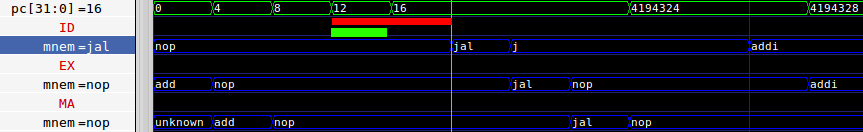
\includegraphics[width=1\textwidth, height=10cm, keepaspectratio]{pictures/task3_delayOfPCInstruction}
	\caption{Delay of PC instruction after 3 nops one JAL command}
	\label{fig3-5}
\end{figure}


%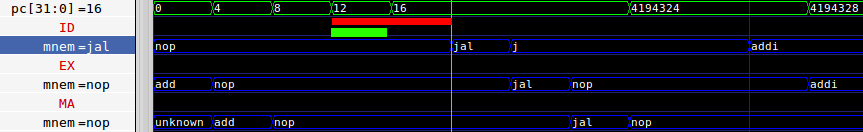
\includegraphics[width=15cm,height=10cm,keepaspectratio]{pictures/task3_delayOfPCInstruction}


%\cacheResultFigure{pictures/task3_delayOfPCInstruction}{Delay of PC instruction after 3 nops one JAL command}
	
Our control logic has to be adapted to the fact that now 4 nops had to be inserted instead of just three and also the program counter had to be frozen accordingly.
The PC freezing logic had to receive the instruction commands as early as possible. Therefore the logic needed to check the opcode of the instruction even before it was written into the first ID register. This way the system could understand when the program counter needs to be kept the same. Inserting nops after a branch or jump command occured in the ID register was not that much of a deal. The only big adaption was the addition of one stalling cycle more. Before the functionality basically was: If a jump or branch command occurs, stall until it reoccurs in MA phase, then set it back to '0' again. Now we needed one more stalling cycle and needed to let the stalling signal be set to '0' if the branch or jump command occured in the WB phase. Unfortunately the control instruction registers were not passed onto the WB phase from the MA phase. Therefore we had to adjust the system and add additional instruction forwarding in the mips\_pkg.vhd file.


TODO insert Mips pkg instruction forward information.

\lstinputlisting[caption={FreezingPC.txt}]{appendix/task3_change5_freezingPC.txt}


\subsection{Additional Details - One Nop at the Beginning Needed}
After our logic was implemented and the test runs were successfull it was interesting to see that some odd behaviour occured at the beginning of the program. It might be important to mention this behaviour in order to clearify   the situation and make bug hunting easier. The first command that is processed by the modified mips is a nop command due to the initialized state.  But it turned out that the second command will be executed twice in a row. In order to bypass this strange behaviour we simply inserted a nop at the beginning of each asm program. The consequence was a doubled nop command, which has no impact on the program at all.

\subsection{Lessons Learned so Far}
Besides the normal lessons like 

\begin{itemize}
\item ``keeping code as simple as possible"
\item ``commenting code pays off''
\item ``divide and conquer problems''
\item ``do testing, testing and testing''
\end{itemize}

another very important lesson was to take into consideration that it takes more time to get things running if team members are using different versions of an operating system or even different operating systems themselves. For instance we had to adapt scripts for windows and linux computers and during some time had different simulation results on our computers, which later on dissvoled after cleaning up temporary files and folders. Still this was quite annoying and took time to dissolve. Reducing the realm of possible error can be a big advantage.




% -----------------------------------------------------
% Documentation regarding task 4.
% -----------------------------------------------------
\newpage
\section{Task 4 - Caches}
\documentclass[11pt,a4paper]{article}

% -----------------------------------------------------
%	Use packages.
% -----------------------------------------------------
\usepackage[german,ngerman]{babel}
\usepackage[utf8]{inputenc}
\usepackage{csquotes}
\usepackage[left=2.5cm,right=3cm,top=3cm,bottom=3cm]{geometry}
\usepackage{subfiles}
\usepackage{helvet}
\usepackage{graphicx}
\usepackage{titling}
\usepackage{blindtext} % Used to generate blindtext.
\usepackage{mathptmx}	% Used for Times New Roman.
\usepackage{bibgerm}
\usepackage[backend=bibtex,style=numeric]{biblatex}  %backend=biber is 'better'  
% backend = {biber, bibtex}
\usepackage{pgf}
\usepackage{tikz}
\usetikzlibrary{arrows,automata}
\usepackage{hyperref}

% -----------------------------------------------------
%	Define attributes.
% -----------------------------------------------------
\title{Advanced System-on-Chip Design}
\author{author}

\definecolor{mycolor}{RGB}{0,65,128}

\newcommand{\cacheResultFigure}[3]{
\begin{figure}
	\centering
	\includegraphics[scale=.8]{#1}
	\caption{#2}
	\label{#3}
\end{figure}
}



% -----------------------------------------------------
%	Add bibliography resources.
% -----------------------------------------------------
%\addbibresource{references.bib}

% =====================================================
\begin{document}

% Include the titelpage.
% !TEX root = fce.tex
% -----------------------------------------------------------------
% Filename  :	titlepage.tex
% Date		:	24/01/2017
% -----------------------------------------------------------------
\begin{titlepage}
	\centering
	
\includegraphics[width=0.30\textwidth]{pictures/office_rgb_en.png}\par\vspace{1cm}
	{\scshape\LARGE Hamburg University of Technology \par}
	\vspace{1cm}
	{\scshape\Large Problem-based Learning\par}
	\vspace{1.5cm}
	{\huge\bfseries \thetitle\par}
	\vspace{1cm}
	{\Large\itshape {Carsten Hoppe} \\\href{mailto:carsten.hoppe@tuhh.de}{carsten.hoppe@tuhh.de}\par}
	\vspace{0.5cm}
	{\Large\itshape Hendrik Meyer zum Felde\\\href{mailto:hendrik.meyer@tuhh.de}{hendrik.meyer@tuhh.de}\par}
	\vspace{.5cm}
	{\Large\itshape Leonard Püttjer \\\href{mailto:leonard.puettjer@tuhh.de}{leonard.puettjer@tuhh.de}\par}
	
	\vfill	% vertikaler Zwischenraum
	Documentation	\\Advanced System on Chip \par
	
	\vfill	% vertikaler Zwischenraum
	Tutor\par
	Dipl.-Ing. Wolfgang \textsc{Brandt}

	\vfill

% Bottom of the page
	{\large \today\par}
\end{titlepage}




% Table of contents.
\tableofcontents
\newpage

% Include introduction.
\section{Cache Simulation - Results}
The two assembler programs \textit{row-major.asm} and \textit{column-major.asm} has been used for the cache simulation. \ref{tab:tableColumnMajor} contains the results regarding the file \textit{column-major.asm} and  \ref{tab:tableRowMajor} illustrates the results of \textit{row-major.asm}.\\
TODO Interpretation



\begin{table}
\centering
\caption{Cache Simulation of Column Major}
\label{tab:tableColumnMajor}
\begin{tabular}{lllll}
\hline %\toprule
Placement (Policy) & Cache Block Size (Words) & Cache Hit Count & Cache Miss Count & Cache Hit Rate \\
\hline %\midrule
Direct Mapping & 2 & 0 & 256 & 0  \\
Direct Mapping & 4 & 0 & 256 & 0  \\
Direct Mapping & 8 & 0 & 256 & 0  \\
Direct Mapping & 16 & 0 & 256 & 0  \\
2-Way Set Associative & 2 & 0 & 256 & 0 \\
2-Way Set Associative & 4 & 0 & 256 & 0 \\
2-Way Set Associative & 8 & 0 & 512 & 0 \\
2-Way Set Associative & 16 & 0 & 256 & 0 \\
4-Way Set Associative & 2 & 0 & 256 & 0 \\
4-Way Set Associative & 4 & 0 & 256 & 0 \\
4-Way Set Associative & 8 & 0 & 256 & 0 \\
4-Way Set Associative & 16 & 0 & 256 & 0 \\
\hline %\bottomrule
\end{tabular} 
\end{table}

\begin{table}
\caption{Cache Simulation of Row Major}
\label{tab:tableRowMajor}
\begin{tabular}{lllll}
\hline %\toprule
Placement (Policy) & Cache Block Size (Words) & Cache Hit Count & Cache Miss Count & Cache Hit Rate \\
\hline %\midrule
Direct Mapping & 2 & 128 & 128 & 50  \\
Direct Mapping & 4 & 192 & 64 & 75  \\
Direct Mapping & 8 & 224 & 32 & 88  \\
Direct Mapping & 16 & 240 & 16 & 94  \\
2-Way Set Associative & 2 & 128 & 128 & 50 \\
2-Way Set Associative & 4 & 192 & 64 & 75 \\
2-Way Set Associative & 8 & 224 & 32 & 88 \\
2-Way Set Associative & 16 & 240 & 16 & 94 \\
4-Way Set Associative & 2 & 128 & 128 & 50 \\
4-Way Set Associative & 4 & 192 & 64 & 75 \\
4-Way Set Associative & 8 & 224 & 16 & 88 \\
4-Way Set Associative & 16 & 240 & 16 & 94 \\
\hline %\bottomrule
\end{tabular} 
\end{table}

\newpage
\section{Design a Finite State Machine for the Cache}

\subsection{Finite State Machine - Write Allocate Policy}
% !TEX root = task4.tex
% -----------------------------------------------------------------
% Filename  :	task4_stateMachine_writeAllocatePolicy.tex
% Author    :	Carsten Hoppe
% Date		:	28. Januar 2017
% Reference	:	http://www.texample.net/tikz/examples/state-machine/
%				https://martin-thoma.com/how-to-draw-a-finite-state-machine/
% -----------------------------------------------------------------
%\tikzstyle{every state}=[fill=mycolor,text=white,minimum width=2cm]
After we have implemented the direct mapped cache, we have to design a finite state machine for the cache controller. This controller have to count the cache hits and cache misses using counters, which are reset at program start. On the one hand, we implement the write back policy. On the other hand, we implement the write allocate policy.\\
In figure \ref{tik:FSM} the state diagram of the cache controller is illustrated. The state diagram represents a Mealy automaton. Besides the state machine inputs are listed in table \ref{tab:tableFSMInputs} and the state machine outputs are shown in table \ref{tab:tableFSMOutputs}. A sketch of the state diagram is printed in figure \ref{fig:sketchMealyAutomata}.\\
In the following, we describe the state space of the state machine:
\begin{itemize}
	\item[IDLE] This state is the initial state of the state machine. When the cache is reset and state machine switches to this state.
	\item[CHECK1] In this state, the cache is checking whether write operation will results in a cache hit or not. Thus, the valid bit, dirty bit and the tag values of the correspondent cache block line are relevant for checking cache hit or cache miss.
	\item[CHECK2] In this state, the cache is checking whether read operation will results in a cache hit or not. Thus, the valid bit, dirty bit and the tag values of the correspondent cache block line are relevant for checking cache hit or cache miss.
	\item[WRITEBACK1] When checking the current cache block line results in a cache miss, and the current cache block line is dirty, this cache block line must be written back to the main memory first. Inside this state, the cache writes the cache block line back to the main memory. The process of writting back requires a specific number of clock cycles. Thus, we have to wait for the main memory. If the main memory signalizes that it is ready, then we can change this state to the next state.
	\item[WRITEBACK2] When checking the current cache block line results in a cache miss, and the current cache block line is dirty, this cache block line must be written back to the main memory first. Inside this state, the cache writes the cache block line back to the main memory. This process of writting back requires a specific number of clock cycles. Thus, we have to wait for the main memory. If the main memory signalizes that it is ready, then we can change this state to the next state.
	\item[WRITE] Before we will write the new data word into the cache, we have to read the cache block line from the main memory into the cache. While the cache is reading from the main memory, we stay in this state. When the main memory is ready and the cache finished reading from the main memory, we switch the current state.
	\item[READ] In case of a cache miss, we have to read the correspondent cache block line from the main memory into the cache. While the we are reading from the main memory, we are inside this state. The main memory signalizes via a correspondent signal if the read operation is finished.
	\item[TOCACHE1] When the write operation has been finished, we achieve this state of the state machine. This state is necessary to increment the miss counter by one. 
	\item[TOCACHE2] When the read operation has been finished, we achieve this state. This state is necessary to increment the miss counter by one. Also, we transmit the requested data word from the cache to the CPU.
\end{itemize}


\newpage
\begin{landscape}
\begin{figure}
	\centering
	\caption{State diagram of the cache controller.}
    \label{tik:FSM}
	\fcolorbox{blue}{myOrange}{
	\begin{tikzpicture}[->,>=stealth',shorten >=1pt,auto,semithick,/tikz/initial text=Reset]
                    
	% ------------------------------------------------------------------------------
    % Definition of tikz styles.       
	% ------------------------------------------------------------------------------
	\tikzstyle{vertex}=[state,fill=mycolor,text=white,minimum width=1cm]
	\tikzstyle{edge}  =[draw,thick,->, midway, above, sloped, font=\tiny]
	\tikzset{invisible/.style={minimum width=0mm,inner sep=0mm,outer sep=0mm}}
	
	% ------------------------------------------------------------------------------
	% Definition of nodes.
	% ------------------------------------------------------------------------------
	[align=center,xscale=1,node distance=2cm and 4cm]
	\node[initial,vertex]	(A)                    		{\tiny $IDLE$};
  	\node[vertex]         	(B) [below  left=5cm of A] 	{\tiny $CHECK1$};
  	\node[vertex]			(C) [below right=5cm of A]	{\tiny $CHECK2$};
  	\node[vertex]         	(D) [below  left=4cm of B] 	{\tiny $WRITEBACK1$};
  	\node[vertex]         	(E) [below right=4cm of C] 	{\tiny $WRITEBACK2$};
  	\node[vertex]         	(F) [below right=4cm of D] 	{\tiny $WRITE$};
  	\node[vertex]			(G) [below  left=4cm of E]  {\tiny $READ$};
  	\node[vertex]		    (H) [below  =2cm of F]  {\tiny $TOCACHE1$};
  	\node[vertex]			(I) [below =2cm of G]  {\tiny $TOCACHE2$};
  	\node	(J) [below =9cm of A,invisible]	{};

	% ------------------------------------------------------------------------------
	% Definition of paths.
	% ------------------------------------------------------------------------------
	\path (A) [edge] 	edge [bend right] node 	{wrCPURequest/-} 	(B)
	      (A) [edge]	edge [bend  left] node  {rdCPURequest/-}	(C)
	      (B) [edge]	edge [bend right] node  {hit/hitCounter++, data2Cache} (A)
	      (C) [edge]	edge [bend left ] node  {hit/hitCounter++, data2CPU} (A)
	      (B) [edge]    edge [bend left ] node  {lineIsNotDirty / rdMEM='1'} (F)
	      (B) [edge]    edge [bend right] node  {lineIsInvalid / rdMEM='1'} (F)
	      (B) [edge]	edge			  node	{lineIsDirty / cacheLine2MEM} (D)
	      (D) [edge]	edge 			  node	{readyMEM / rdMEM='1'} (F)
	      (F) [edge]	edge			  node	{readyMEM / wrNewCBLine} (H)
	      (H) [edge] 	edge [bend right] node 	{- / missCounter++, data2Cache} (J)
	      (C) [edge]	edge 			  node  {lineIsDirty / cacheLine2MEM} (E)
	      (C) [edge]	edge [bend right] node  {lineIsInvalid / rdMEM='1'} (G)
	      (C) [edge]	edge [bend left ] node  {lineIsNotDirty / rdMEM='1'} (G)
	      (E) [edge]	edge 			  node	{readyMEM / -} (G)
	      (I) [edge]	edge [bend left ] node	{- / missCounter++, data2CPU} (J)
	      (G) [edge]	edge 			  node  {readyMEM / -} (I)
	      (J) [edge]	edge 			  node  {} (A)
	      (E) [edge,loop right] edge	  node  {!readyMEM / -} (E)
	      (G) [edge,loop left]  edge	  node  {!readyMEM / -} (G)
	      (D) [edge,loop left] edge 	  node	{!readyMEM / -} (D)
	      (F) [edge,loop right] edge	  node  {!readyMEM / -} (F);
	      		
\end{tikzpicture}}
\end{figure}
\end{landscape}
\newpage

\begin{table}
	\caption{Overview - FSM Inputs}
	\label{tab:tableFSMInputs}
	\begin{tabular}{lll}
	\hline % \topline
	Abbreviation & Name & Description \\
	\hline % \midrule
	rdCPU 		& CPU Read Request			& - \\
	wrCPU 		& CPU Write Request 		& - \\
	cacheMiss 	& Cache Miss 				& - \\
	cacheHit	& Cache Hit					& - \\
	readyMEM 	& Write-Back is resolved 	& - \\
	isDirty		& Cache Block is dirty		& - \\
	\hline % \bottomrule
	\end{tabular}
\end{table}
	
\begin{table}
	\caption{Overview - FSM Outputs}
	\label{tab:tableFSMOutputs}
	\begin{tabular}{lll}
	\hline % \topline
	Abbreviation & Name & Description \\
	\hline % \midrule
	stallCPU		& Stall Processor				& - \\
	setDirty		& Set Dirty Bit (Modified) Bit 	& - \\
	wrMEM			& Write To Memory				& Write Replaced Block To Memory \\
	dataCPU			& Read Data Into CPU			& - \\
	rdMEM			& Read Cache Block Into Cache From Memory & - \\
	dataCPU2Cache	& Write Data Into Cache			& - \\
	\hline % \bottolrule
	\end{tabular}
\end{table}

\newpage
\begin{landscape}
\begin{figure}
	\centering
	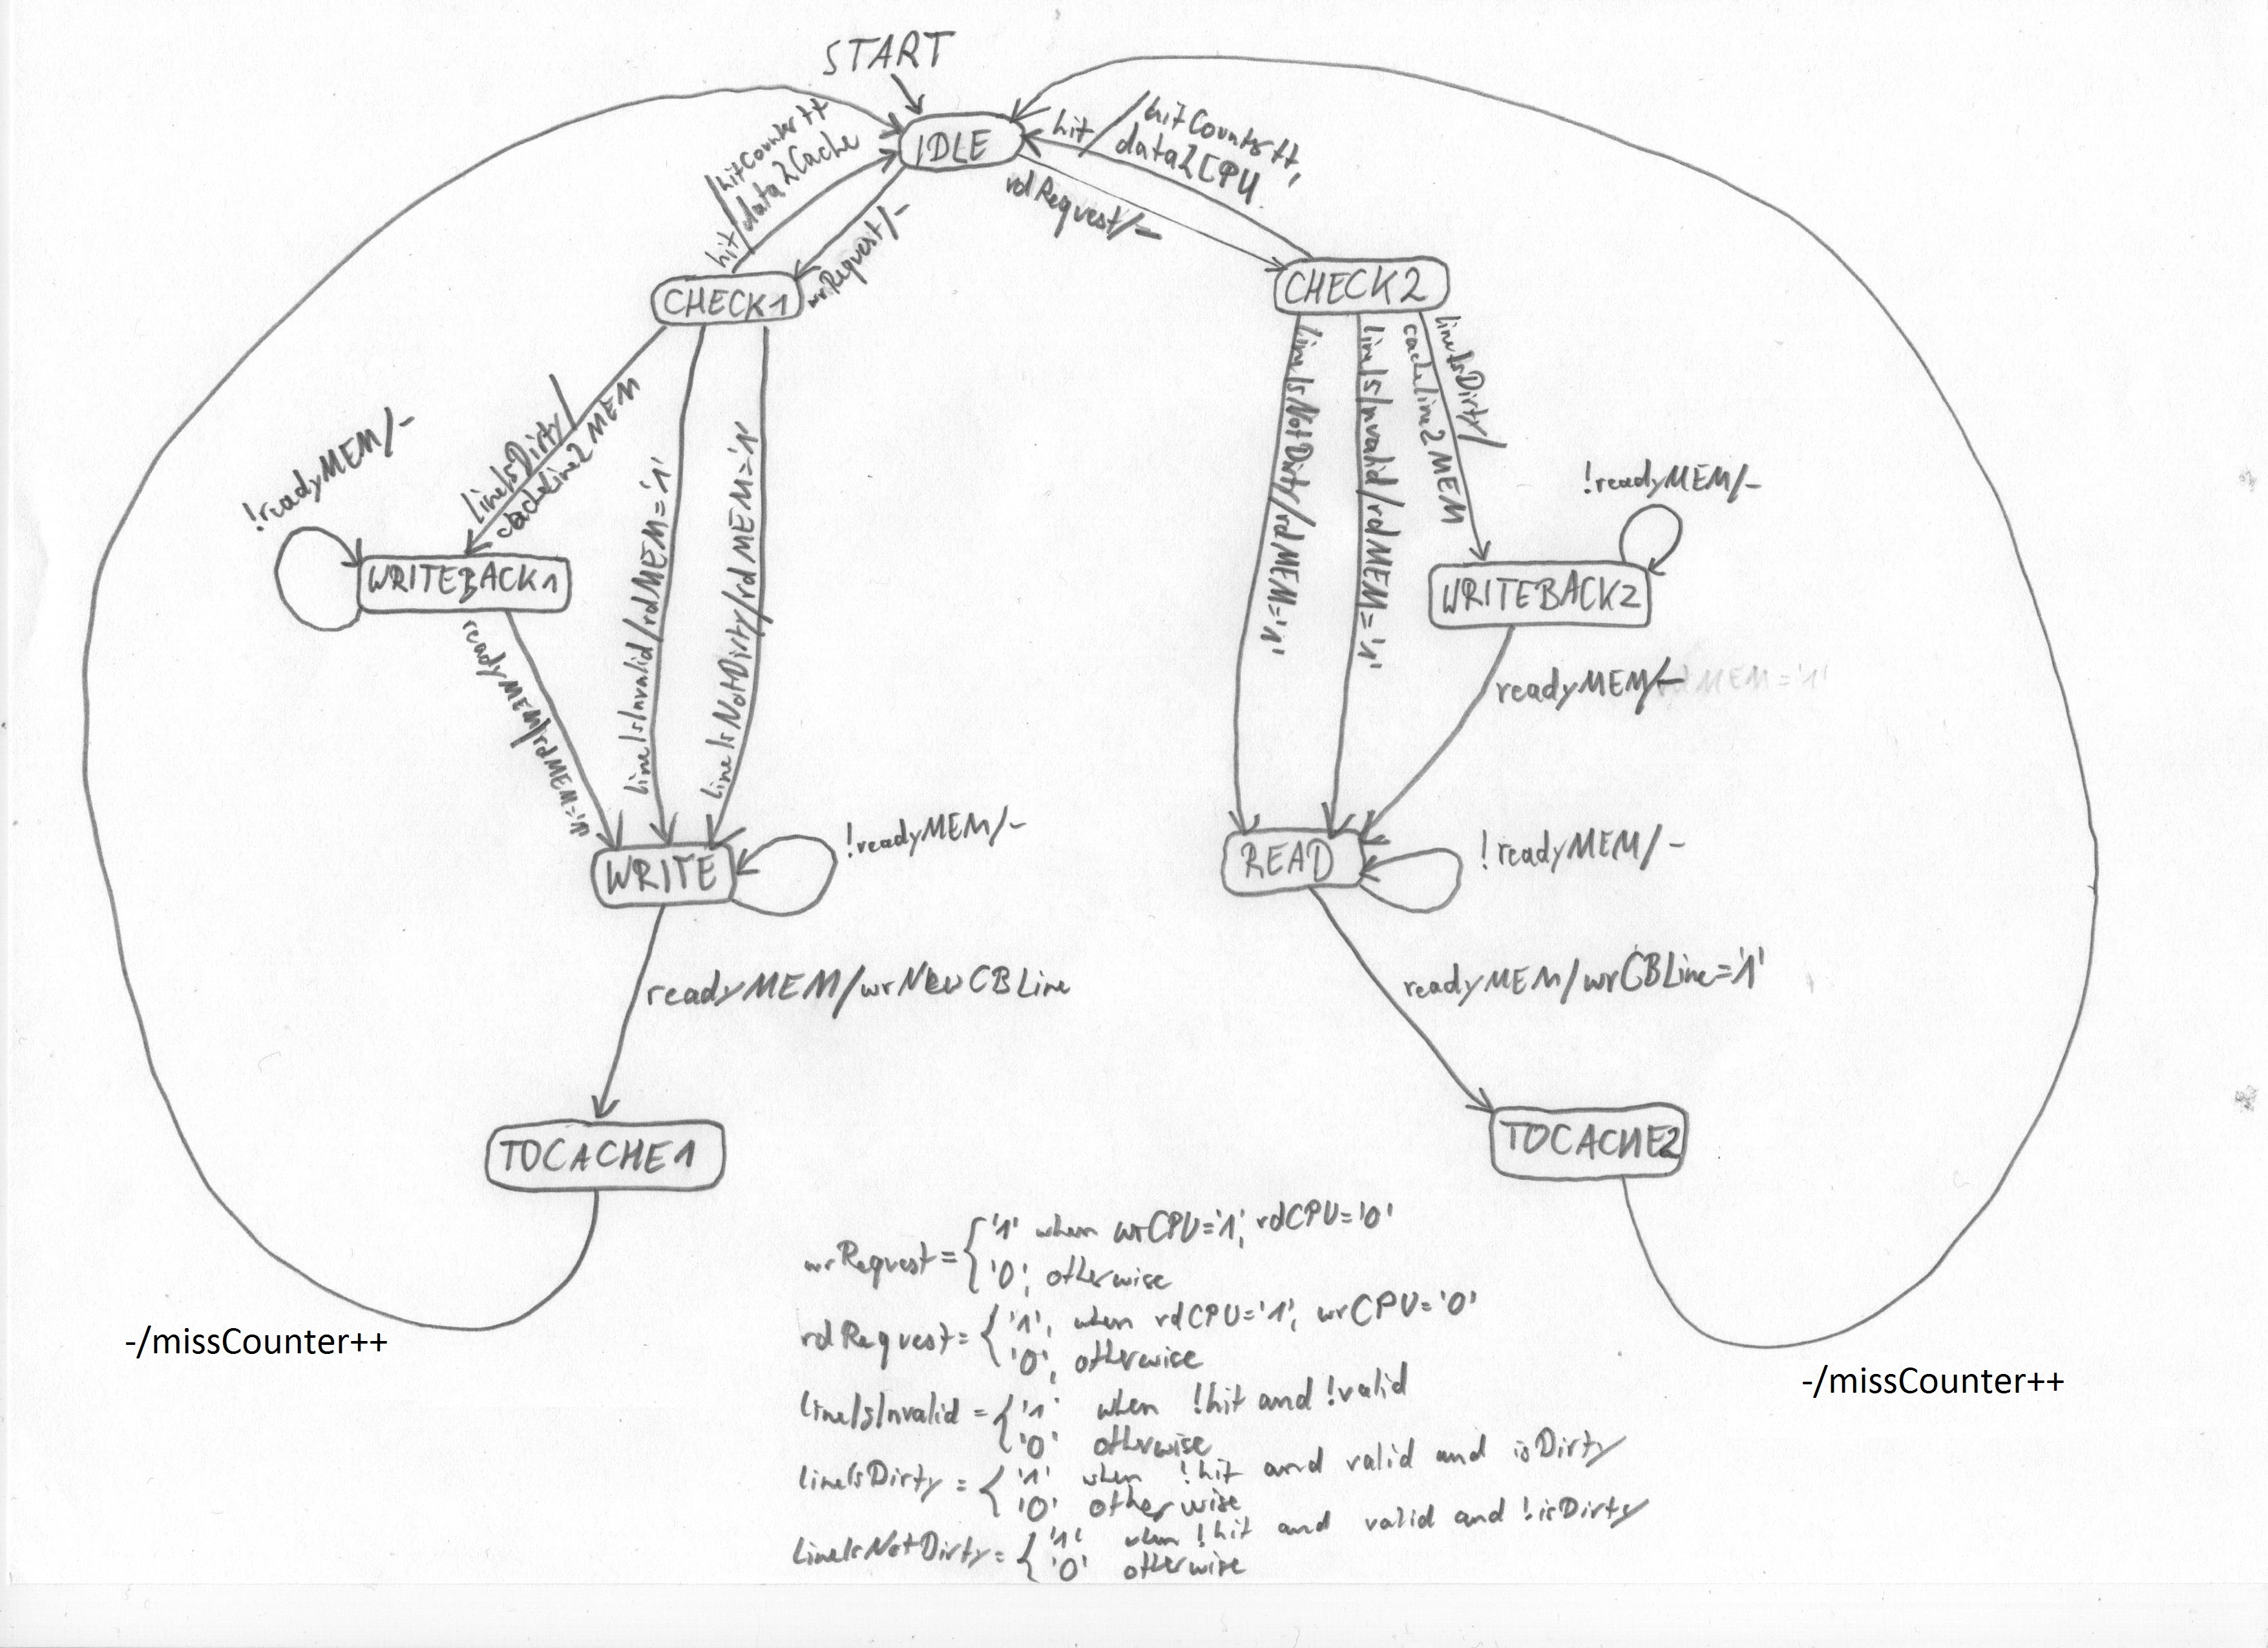
\includegraphics[scale=.8]{pictures/sketch_mealyAutomata_v2_modified}
	\caption{Sketch of Mealy Automata - Cache Controller, Version 2}
	\label{fig:sketchMealyAutomata}
\end{figure}
\end{landscape}

\subsection{Finite State Machine - Example}
% !TEX root = task4.tex
% -----------------------------------------------------------------
% Filename  :	example_stateMachine.tex
% Author    :	Carsten Hoppe
% Date		:	28. Januar 2017
% Reference	:	http://www.texample.net/tikz/examples/state-machine/
%				https://martin-thoma.com/how-to-draw-a-finite-state-machine/
% -----------------------------------------------------------------

\begin{tikzpicture}[->,>=stealth',shorten >=1pt,auto,node distance=2.8cm,
                    semithick]
  \tikzstyle{every state}=[fill=red,draw=none,text=white]

  \node[initial,state] (A)                    {$q_a$};
  \node[state]         (B) [above right of=A] {$q_b$};
  \node[state]         (D) [below right of=A] {$q_d$};
  \node[state]         (C) [below right of=B] {$q_c$};
  \node[state]         (E) [below of=D]       {$q_e$};

  \path (A) edge              node {0,1,L} (B)
            edge              node {1,1,R} (C)
        (B) edge [loop above] node {1,1,L} (B)
            edge              node {0,1,L} (C)
        (C) edge              node {0,1,L} (D)
            edge [bend left]  node {1,0,R} (E)
        (D) edge [loop below] node {1,1,R} (D)
            edge              node {0,1,R} (A)
        (E) edge [bend left]  node {1,0,R} (A);
\end{tikzpicture}










\newpage
\section{Appendix}
\cacheResultFigure{pictures/task4_columnMajor_directMapping2}{Column Major, Direct Mapping, Cache Block Size 2}{fig:pic}
\cacheResultFigure{pictures/task4_columnMajor_directMapping4}{Column Major, Direct Mapping, Cache Block Size 4}{fig:pic}
\cacheResultFigure{pictures/task4_columnMajor_directMapping8}{Column Major, Direct Mapping, Cache Block Size 8}{fig:pic}
\cacheResultFigure{pictures/task4_columnMajor_directMapping16}{Column Major, Direct Mapping, Cache Block Size 16}{fig:pic}

\cacheResultFigure{pictures/task4_columnMajor_2waySetAssociative2}{Column Major, 2-Way Associative, Cache Block Size 2}{fig:pic}
\cacheResultFigure{pictures/task4_columnMajor_2waySetAssociative4}{Column Major, 2-Way Associative, Cache Block Size 4}{fig:pic}
\cacheResultFigure{pictures/task4_columnMajor_2waySetAssociative8}{Column Major, 2-Way Associative, Cache Block Size 8}{fig:pic}
\cacheResultFigure{pictures/task4_columnMajor_2waySetAssociative16}{Column Major, 2-Way Associative, Cache Block Size 16}{fig:pic}

\cacheResultFigure{pictures/task4_columnMajor_4waySetAssociative2}{Column Major, 4-Way Associative, Cache Block Size 2}{fig:pic}
\cacheResultFigure{pictures/task4_columnMajor_4waySetAssociative4}{Column Major, 4-Way Associative, Cache Block Size 4}{fig:pic}
\cacheResultFigure{pictures/task4_columnMajor_4waySetAssociative8}{Column Major, 4-Way Associative, Cache Block Size 8}{fig:pic}
\cacheResultFigure{pictures/task4_columnMajor_4waySetAssociative16}{Column Major, 4-Way Associative, Cache Block Size 16}{fig:pic}


\cacheResultFigure{pictures/task4_rowMajor_directMapping2}{Row Major, Direct Mapping, Cache Block Size 2}{fig:pic}
\cacheResultFigure{pictures/task4_rowMajor_directMapping4}{Row Major, Direct Mapping, Cache Block Size 4}{fig:pic}
\cacheResultFigure{pictures/task4_rowMajor_directMapping8}{Row Major, Direct Mapping, Cache Block Size 8}{fig:pic}
\cacheResultFigure{pictures/task4_rowMajor_directMapping16}{Row Major, Direct Mapping, Cache Block Size 16}{fig:pic}

\cacheResultFigure{pictures/task4_rowMajor_2waySetAssociative2}{Row Major, 2-Way Associative, Cache Block Size 2}{fig:pic}
\cacheResultFigure{pictures/task4_rowMajor_2waySetAssociative4}{Row Major, 2-Way Associative, Cache Block Size 4}{fig:pic}
\cacheResultFigure{pictures/task4_rowMajor_2waySetAssociative8}{Row Major, 2-Way Associative, Cache Block Size 8}{fig:pic}
\cacheResultFigure{pictures/task4_rowMajor_2waySetAssociative16}{Row Major, 2-Way Associative, Cache Block Size 16}{fig:pic}

\cacheResultFigure{pictures/task4_rowMajor_4waySetAssociative2}{Row Major, 4-Way Associative, Cache Block Size 2}{fig:pic}
\cacheResultFigure{pictures/task4_rowMajor_4waySetAssociative4}{Row Major, 4-Way Associative, Cache Block Size 4}{fig:pic}
\cacheResultFigure{pictures/task4_rowMajor_4waySetAssociative8}{Row Major, 4-Way Associative, Cache Block Size 8}{fig:pic}
\cacheResultFigure{pictures/task4_rowMajor_4waySetAssociative16}{Row Major, 4-Way Associative, Cache Block Size 16}{fig:pic}





% Abbildungsverzeichnis
% Abkürzungsverzeichnis
% Verzeichnis der Anhänge
% Anhänge und Materialien

% Include bibliography.
\newpage
\nocite{*}
\printbibliography

% =====================================================
\end{document}

% -----------------------------------------------------
% Documentation regarding task 4.
% -----------------------------------------------------
\newpage
\section{Task 5 - Branch Prediction}
% !TEX root = fce.tex
% -----------------------------------------------------------------
% Filename  :	task5.tex
% Author    :	Meyer zum Felde, Püttjer, Hoppe
% Date		:	18.03.2017
% -----------------------------------------------------------------

\subsection{Branch Prediciton}
\label{sec:branchPrediction}

The task was to implement a branch prediction unit in three ways:

\begin{itemize}
\item ``Static branch prediction''
\item ``Dynamic branch prediction using a branch history table (BHT)''
\item ``dynamic branch prediction using a branch target buffer (BTB)''
\end{itemize}

\subsection{Static Branch Prediciton}
\label{sec:staticBranchPrediction}

For our static branch prediction we needed perform the check if a branch will be taken in the ID phase. The comfortable restriction that was given was the fact that we only need to handle the commands BNE and BEQ since they were the ones used for testing programs like isort\_pipe. In fact no other assembler file given was using other branch commands. Therefore our branch predicition only needed to handle a comparison check of two given registers. This was implemented using the following technique. 

We inserted a new signal called branchIdPhase. This signal was set to 1 whenever a BEQ or BNE command was detected in the ID phase and simultaneously not in MA or EX phase. We wanted it to be set to '1' in order to mark the arrival of a new branch command. Simultenously our signal predictionError receives the input to perform static jumping if our StaticBranchAlwaysTaken signal is set to '1' and the branch condition is not met. In other words if we assume a branch is always taken and the condition to take a branched step is not given our predictionError signal is set to '1'. Whenever we have a predictionError we decide to take another path than the one that was predicted.

\lstinputlisting[caption={BranchCheckMovedToIDPhase}]{appendix/task5_change1_frontAdded.txt}

The impact of our code was to let the system assume a certain strategy like always ``always assume to take a branch'' and performing stalling whenever the prediction was not right. We needed to test whether this strategy was running as well as the possibility to switch the strategy at any time since the logic would be used in the dynamic branching also.


\subsection{Dynamic Branch Prediction Using a BHT}
\label{sec:dynamicBranchPredictionUsingBHT}

In the beginning understanding of the functionality of a BHT needed to be gained. This was done by using the preinstalled feature from the MARS simulator. 
Which can be seen in figure \ref{fig5-1} on page \pageref{fig5-1}.

\begin{figure}
	\centering
  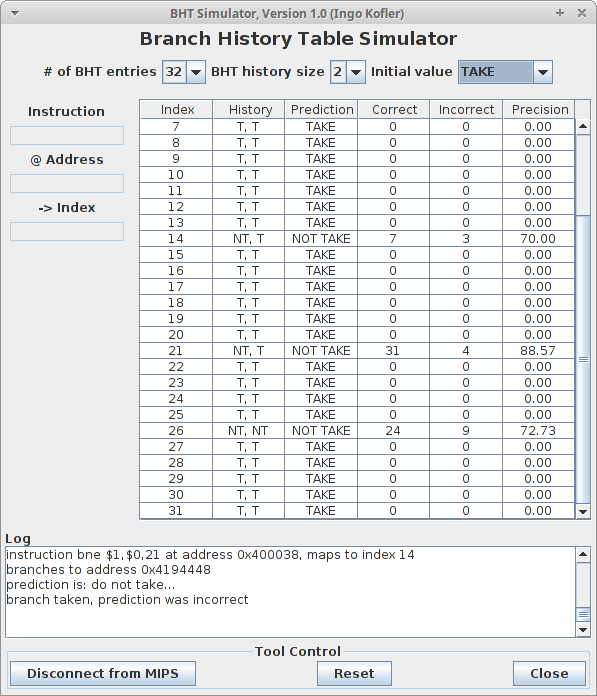
\includegraphics[width=1\textwidth, keepaspectratio]{pictures/task5_BHT_sim_1}
	\caption{Screenshot of BHT Simulation in MARS using isort\_pipe from lecture}
	\label{fig5-1}
\end{figure}

The BHT basically uses a slot for each branch command and remembers the last one or two jumping behaviours. According to the history the next jump should be taken in order to guess as many tries as possible correctly. Our problem is that whenenver we guess our branch jump behaviour wrong, we lose clock cycles. Therefore we want a prediction rate as high as possible. 

The interesting thing is if we compare values for changed input like Intitial state either ``TAKE'' or ``NOT TAKE'' and History size is either 2 or only 1 entry we can see following behaviour in table \ref{tab5-1} on page \pageref{tab5-1}. Additional screenshots of results can be seen in the appendix.

\begin{table}[h]
\resizebox{1\textwidth}{!}{\begin{minipage}{\textwidth}
\begin{tabular}{ l l l l l }
 \hline
 BHT Settings & 1BNE Precision & 2BNE Precision & BEQ Precision\\ \hline

 BHT with History 1 Initial TAKE & 80\% & 88.57\% & 72.73\% \\
 BHT with History 2 Initial TAKE & 70\% & 88.57\% & 72.73\% \\
 BHT with History 1 Initial NOT TAKE & 90\% & 91.43\% & 69.70\% \\
 BHT with History 2 Initial NOT TAKE & 90\% & 94.29\% &75.76\% \\
	\hline
\end{tabular}
\caption[Table caption text]{of successful prediction using BHT in isort\_pipe}
\label{tab5-1}
\end{minipage} }
\end{table}



After creating a running Static branch prediction in the previous task it was afterwards possible to give this branch prediction dynamic inputs. Since static always taken as well as static never taken were modes that could be selected.  Figure \ref{fig5-1} on page \pageref{fig5-1} shows how the prediction of a branch command is compared to the real result and influences the program flow. The vertical red line shows the state of a falling edge at which the variable a and b are compared whether they are equal or not equal in the ID phase. Hald a clock cycle later the result is at hand. Since the Prediction from the BHT says the branch is not taken and the values of a and b are equal to each other and we have a BNE (branch when not equal) command we see that the system will not perform a branch jump. The area of a distance of half a clock cycle to the right of the vertical red marker is not of importance for our logic since it reads out the prediction error of the next PC, instructed by the yellow signal at the top of the screenshot because it will be read at a later state. The read signals show that its BHT status has switched from weakly not taken into strongly not taken.

\begin{figure}
	\centering
	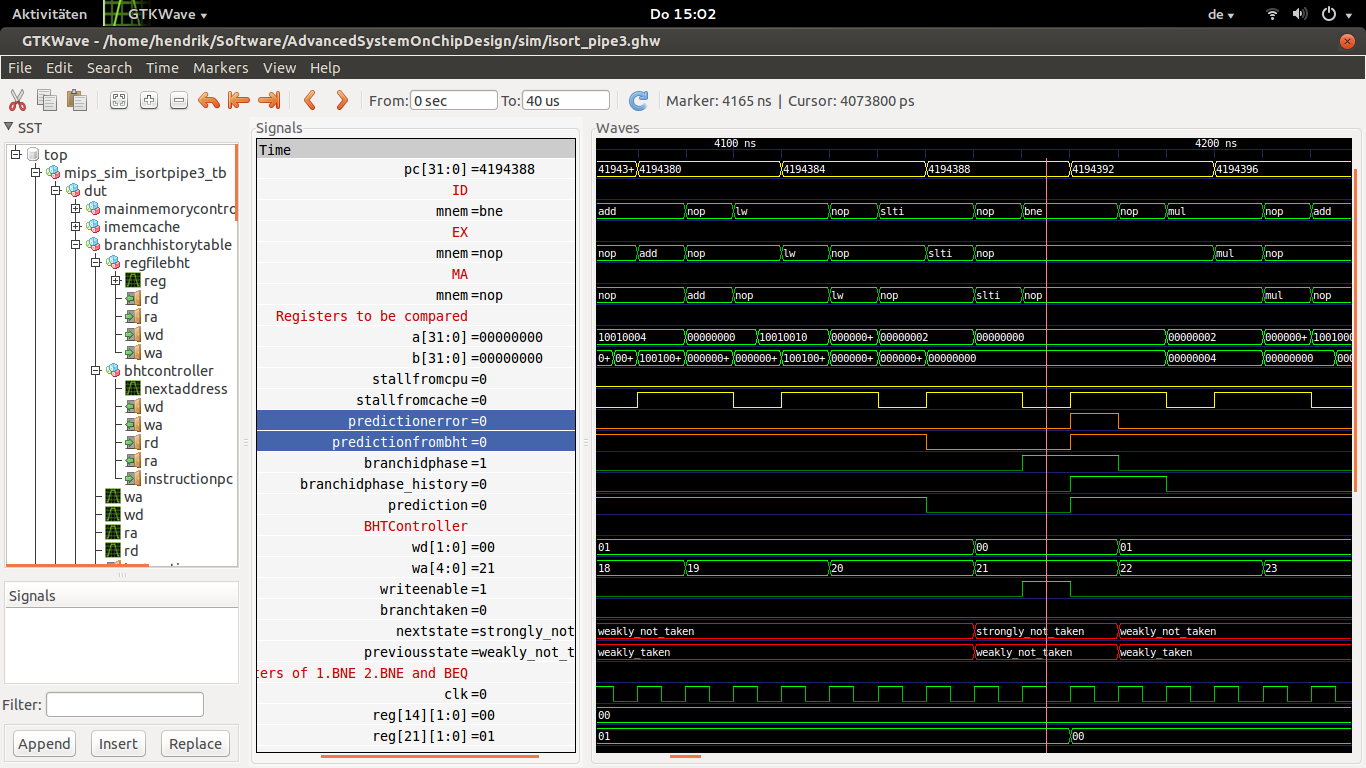
\includegraphics[width=1\textwidth, height=10cm, keepaspectratio]{pictures/BHT_BranchNotTakenPred0Err0}
	\caption{Behaviour of BHT without prediction error}
	\label{fig5-1}
\end{figure}

Figure \ref{fig5-2} on page \pageref{fig5-2} shows a situation where the BHT predicts that the Branch command BEQ will not be taken but actually it will be taken. Its BHT status switches from weakly not taken to weakly taken.


\begin{figure}
	\centering
	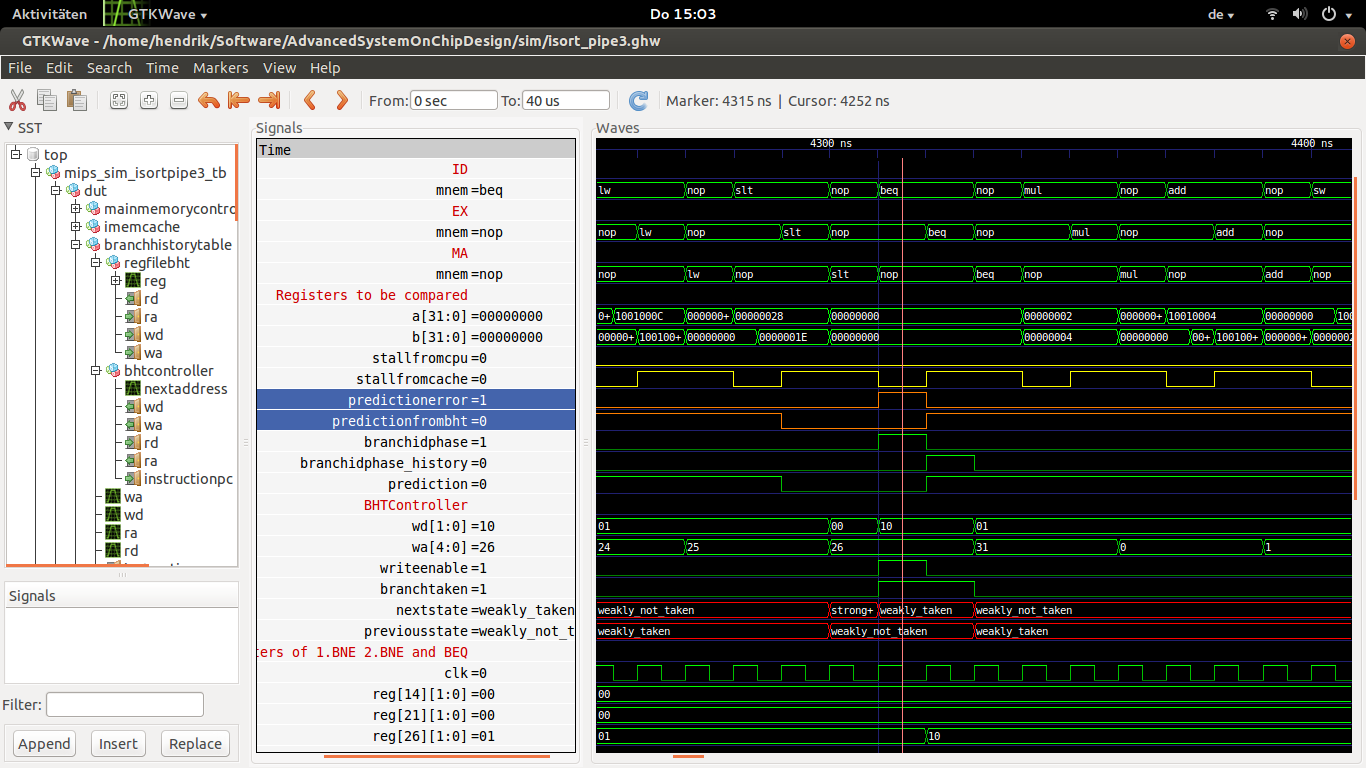
\includegraphics[width=1\textwidth, height=10cm, keepaspectratio]{pictures/BHT_BranchTakenPred0Err1}
	\caption{Behaviour of BHT with prediction error}
	\label{fig5-2}
\end{figure}




\subsection{Dynamic Branch Prediction using BTB}
We wanted to let our mips use a Branch Target Buffer which keeps track of all taken branches and their target Program Counters. In figure \ref{fig5-3} on page \pageref{fig5-3} we can see how a jump command is executed for the first time and its target is saved into the BTB. In figure \ref{fig5-4} on page \pageref{fig5-4} we can see how the process of another jump command which is processed later on is increased in speed because the command has been taken a previous time and the BTB still remembers which target adress it was using. The BTB can be read combinatorically whereas the writing process of writing into the BTB is clock cycle dependant.

\begin{figure}
	\centering
	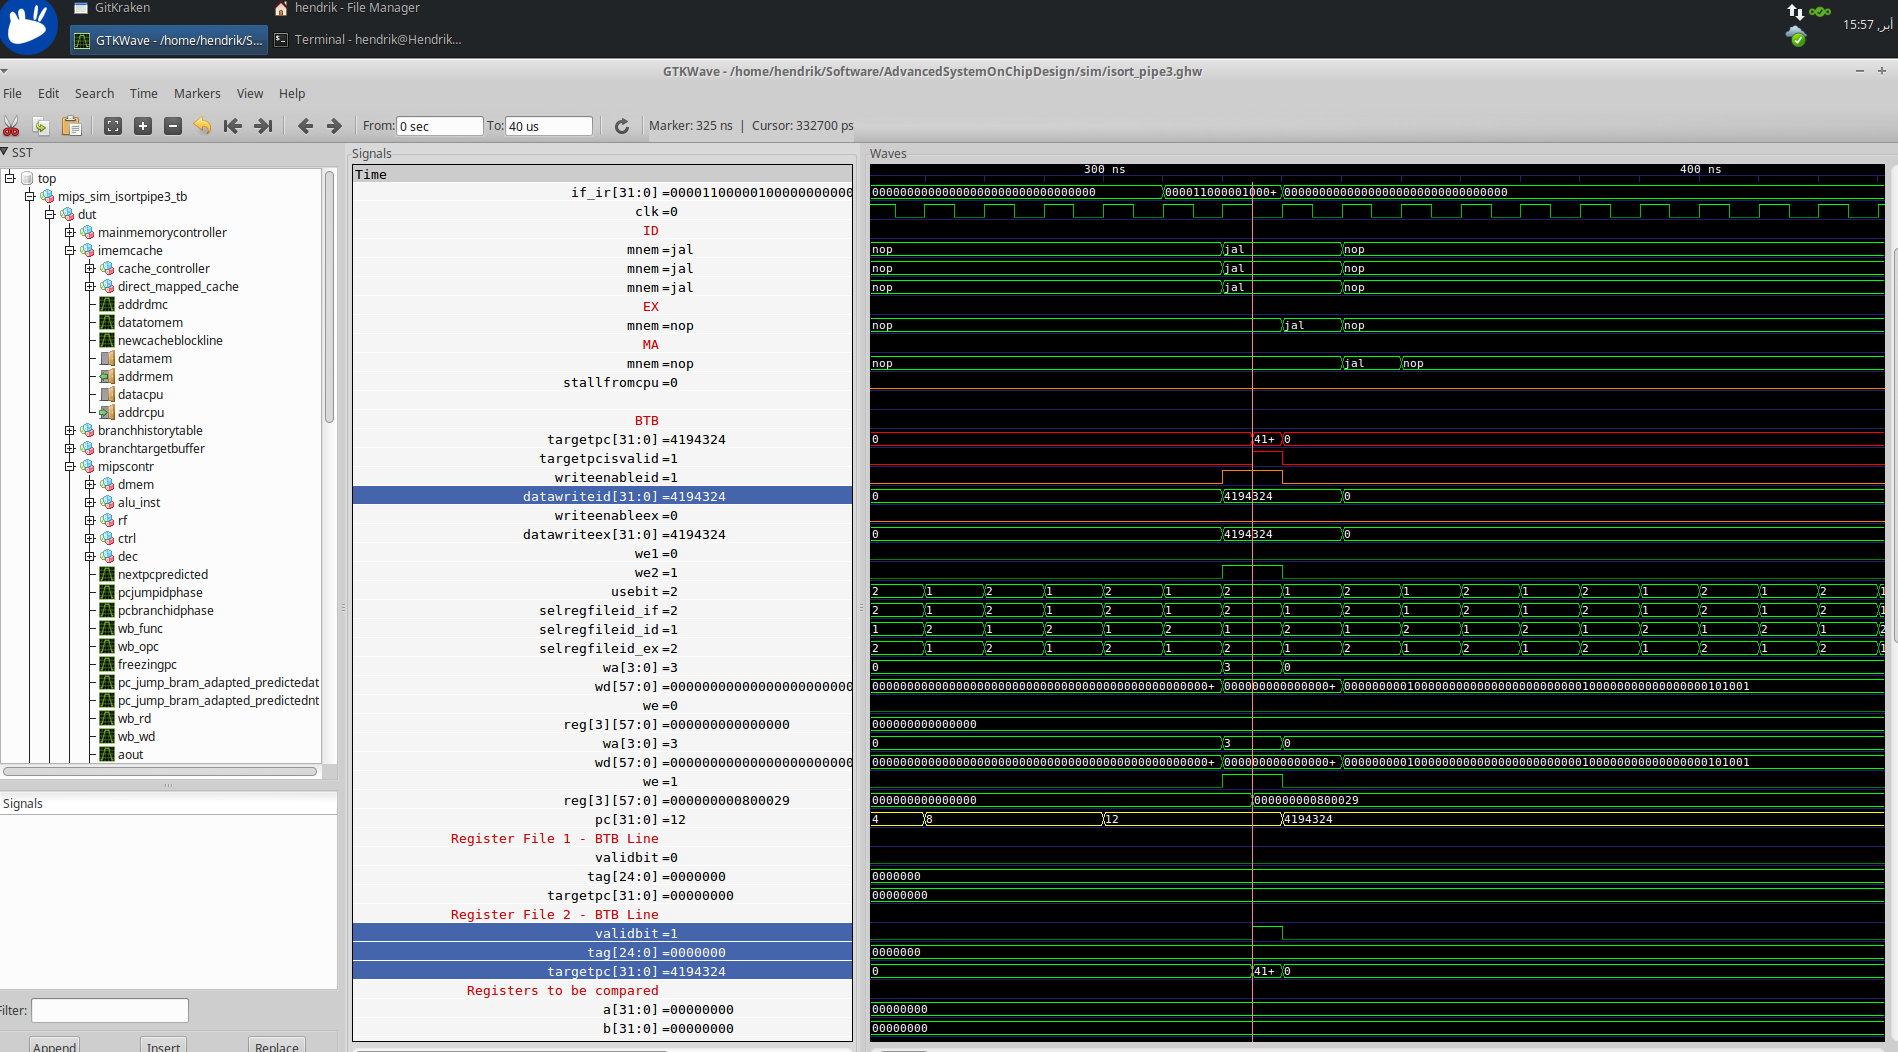
\includegraphics[width=1\textwidth, height=10cm, keepaspectratio]{pictures/BTB_FirstJump}
	\caption{GTKWAVE Screenshot of BTB saving a jump's target at a falling edge}
	\label{fig5-3}
\end{figure}

\begin{figure}
	\centering
	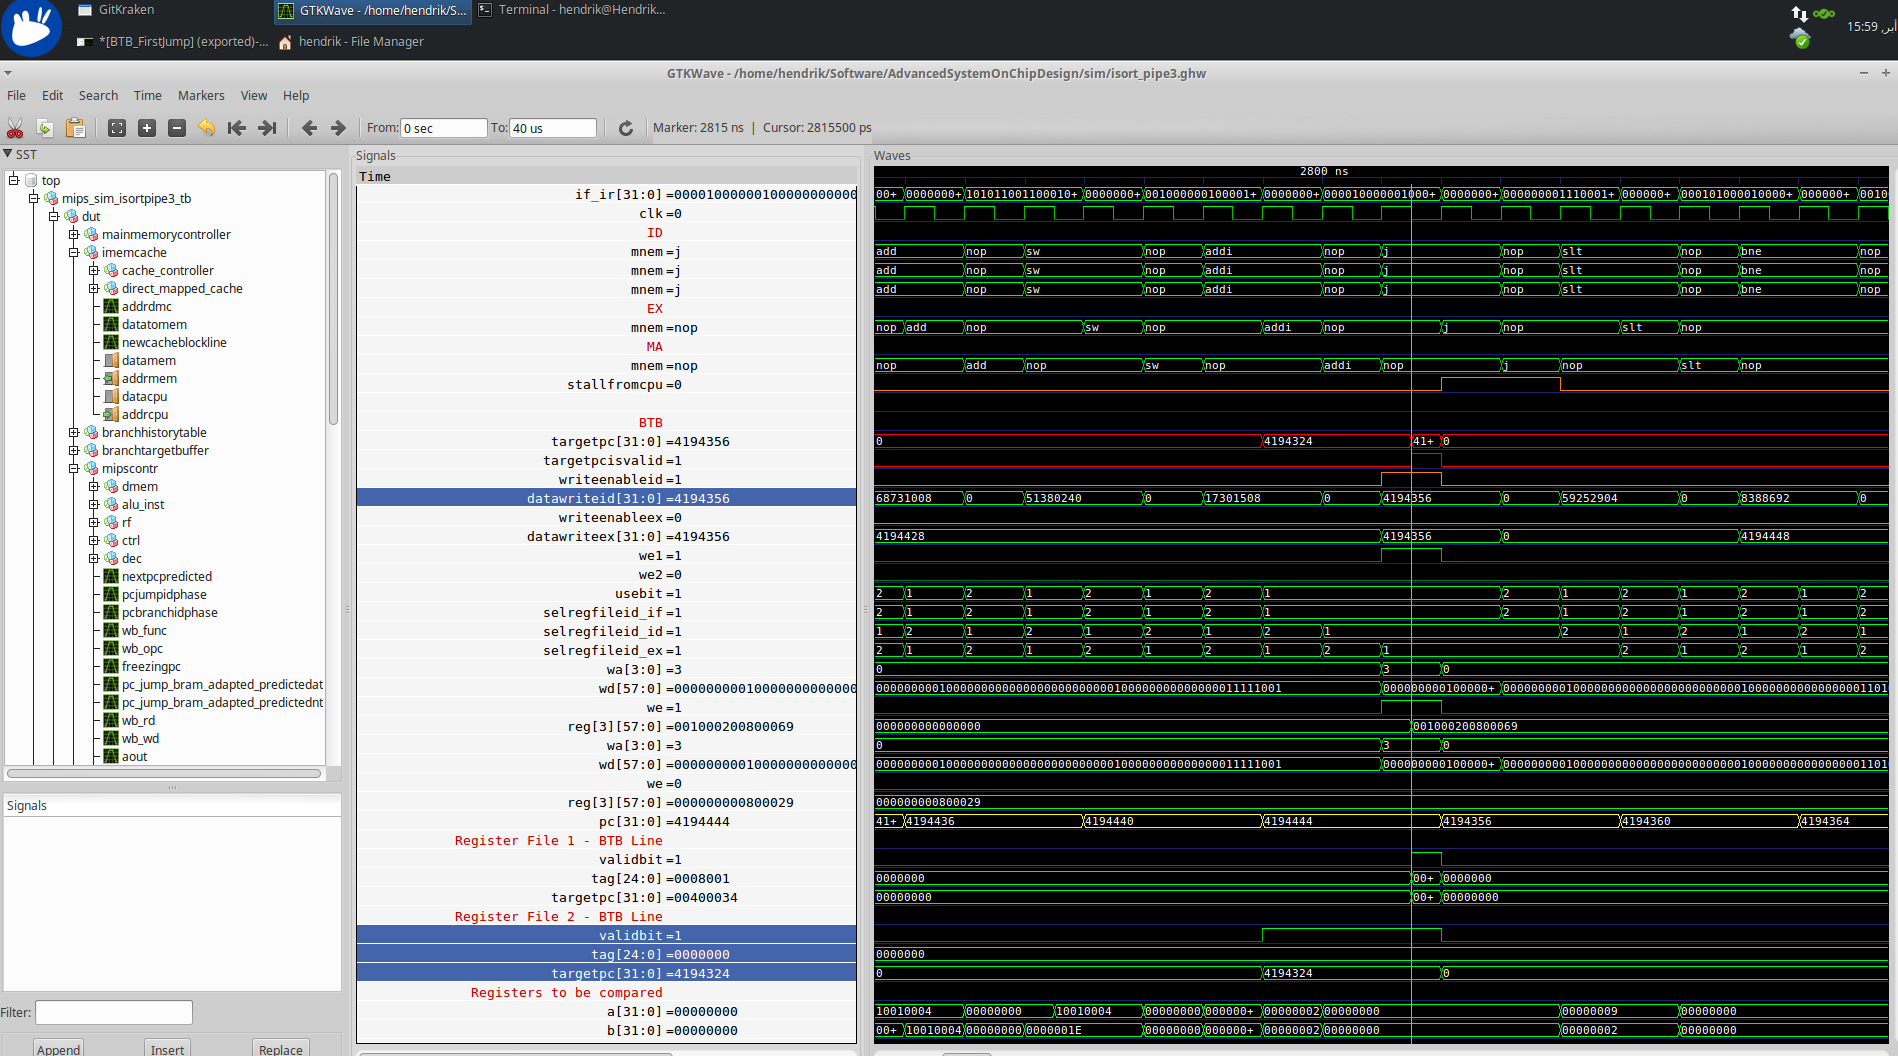
\includegraphics[width=1\textwidth, height=10cm, keepaspectratio]{pictures/BTB_SecondJump}
	\caption{GTKWAVE Screenshot of a jump predicted from BTB}
	\label{fig5-4}
\end{figure}




\subsection{Lessons Learned}
Wnile doing the work of this section another problem occured. Since we were three people using three different OS one of our computers was not able to accept a correct Eclipse Sigasi Certificate on an emulated Linux machine running on a physical Macbook. The workaround at hand was to implement the code on the Mac OS, upload the code using github and pulling the modified  state on the virtual Linux machine. Tests were run in the virtual box but the coding had to be done on the physical OS. This was a bit of a slow down factor since each change of code caused a push and pull action for this team member. We recommend again to use the same OS on all systems and the same Development Software on all machines. For our case we needed some workarounds.


% -----------------------------------------------------
% Documentation regarding task 4.
% -----------------------------------------------------
\newpage
\section{Summary}
% !TEX root = fce.tex
% -----------------------------------------------------------------
% Filename  :	summary.tex
% Author    :	Carsten Hoppe
% Date		:	31. January 2017
% -----------------------------------------------------------------

\subsection{How to Use the Scripts and Testbenches}
\label{sec:howToUseScripts}

After having answered different questions at different stages of the development process of our mips it turned out that a system to easily run and test new as well as old configurations of the mips was necessary. Simply switching between states within the repository was not fully satisfying our needs. Therefore a specified testbench for each program was created with corresponding configurations to chose from.



%TODO in order to test test run MYMARS Varable needs to be adapted either using path variable or inside the 4 run_ghdl_mips_[ isortpipe3 | gcd | fib | fac ]_[linux.sh | %windows.bat]


\begin{itemize}
	\item Configuration1 is mips with pipelining, stalling and forwarding
	\item Configuration2 is Configuration1 with instruction cache
	\item Configuration3 is Configuration2 with static branch prediction
	\item Configuration4 is Configuration3 with Branch History Table implemented
	\item Configuration5 is Configuration4 with Branch Target Buffer implemented
\end{itemize}





\begin{table}[h]
	\resizebox{1\textwidth}{!}{\begin{minipage}{\textwidth}
			\begin{tabular}{ l l l l l l }
				\hline
				Test program & Config c1 & Config c2 & Config c3 & Config c4 & Config c5\\ \hline
				
				FAC	 	& - & OKAY & OKAY & OKAY \\
				FIB 	& - & OKAY & OKAY & OKAY  \\
				GCD 	& - & OKAY & OKAY & OKAY  \\
				ISORT\_PIPE3 & OKAY & OKAY & OKAY & OKAY \\
				\hline
			\end{tabular}
			\caption[Table caption text]{Table showing successful testing events}
			\label{tab5-1}
		\end{minipage} }
	\end{table}

\begin{table}[h]
	\resizebox{1\textwidth}{!}{\begin{minipage}{\textwidth}
			\begin{tabular}{ l l l l l l }
				\hline
				Test program & Config c1 & Config c2 & Config c3 & Config c4 & Config c5\\ \hline
				
				FAC	 	& cfac1 & cfac2 & cfac3 & cfac4 & cfac5 \\
				FIB 	& cfib1 & cfib2 & cfib3 & cfib4 & cfib5 \\
				GCD 	& cgcd1 & cgcd2 & cgcd3 & cgcd4 & cgcd5 \\
				ISORT\_PIPE3 & cisort1 & cisort2 & cisort3 & cisort4 & cisort5 \\
				\hline
			\end{tabular}
			\caption[Table caption text]{Table showing command parameters to call run\_ghdl\_mips\_xxx\_script}
			\label{tab5-1}
		\end{minipage} }
	\end{table}

The corresponding windows and linux scripts in the hdl folder to call with parameter from above are presented here.  
\begin{itemize}
\item  run\_ghdl\_mips\_fac\_linux.sh
\item  run\_ghdl\_mips\_fac\_windows.bat
\item  run\_ghdl\_mips\_fib\_linux.sh
\item  run\_ghdl\_mips\_fib\_windows.bat
\item  run\_ghdl\_mips\_gcd\_linux.sh
\item  run\_ghdl\_mips\_gcd\_windows.bat
\item  run\_ghdl\_mips\_isortPipe3\_linux.sh
\item  run\_ghdl\_mips\_isortPipe3\_windows.bat
\end{itemize}
 
 
 








% -----------------------------------------------------
% Appendix of documentation.
% -----------------------------------------------------
\newpage
\pagestyle{scrheadings}
\section{Appendix}
% !TEX root = fce.tex
% -----------------------------------------------------------------
% Filename  :	appendix.tex
% Author    :	Carsten Hoppe
% Date		:	30. January 2017
% Reference	:	http://www.texample.net/tikz/examples/state-machine/
%				https://martin-thoma.com/how-to-draw-a-finite-state-machine/
% -----------------------------------------------------------------
\subsection{Finite State Machine - Example}
% !TEX root = task4.tex
% -----------------------------------------------------------------
% Filename  :	example_stateMachine.tex
% Author    :	Carsten Hoppe
% Date		:	28. Januar 2017
% Reference	:	http://www.texample.net/tikz/examples/state-machine/
%				https://martin-thoma.com/how-to-draw-a-finite-state-machine/
% -----------------------------------------------------------------

\begin{tikzpicture}[->,>=stealth',shorten >=1pt,auto,node distance=2.8cm,
                    semithick]
  \tikzstyle{every state}=[fill=red,draw=none,text=white]

  \node[initial,state] (A)                    {$q_a$};
  \node[state]         (B) [above right of=A] {$q_b$};
  \node[state]         (D) [below right of=A] {$q_d$};
  \node[state]         (C) [below right of=B] {$q_c$};
  \node[state]         (E) [below of=D]       {$q_e$};

  \path (A) edge              node {0,1,L} (B)
            edge              node {1,1,R} (C)
        (B) edge [loop above] node {1,1,L} (B)
            edge              node {0,1,L} (C)
        (C) edge              node {0,1,L} (D)
            edge [bend left]  node {1,0,R} (E)
        (D) edge [loop below] node {1,1,R} (D)
            edge              node {0,1,R} (A)
        (E) edge [bend left]  node {1,0,R} (A);
\end{tikzpicture}

\subsection{Cache Results - Snapshots}
\cacheResultFigure{pictures/task4_columnMajor_directMapping2}{Column Major, Direct Mapping, Cache Block Size 2}{fig:pic1}
\cacheResultFigure{pictures/task4_columnMajor_directMapping4}{Column Major, Direct Mapping, Cache Block Size 4}{fig:pic2}
\cacheResultFigure{pictures/task4_columnMajor_directMapping8}{Column Major, Direct Mapping, Cache Block Size 8}{fig:pic3}
\cacheResultFigure{pictures/task4_columnMajor_directMapping16}{Column Major, Direct Mapping, Cache Block Size 16}{fig:pic4}

\cacheResultFigure{pictures/task4_columnMajor_2waySetAssociative2}{Column Major, 2-Way Associative, Cache Block Size 2}{fig:pic5}
\cacheResultFigure{pictures/task4_columnMajor_2waySetAssociative4}{Column Major, 2-Way Associative, Cache Block Size 4}{fig:pic6}
\cacheResultFigure{pictures/task4_columnMajor_2waySetAssociative8}{Column Major, 2-Way Associative, Cache Block Size 8}{fig:pic7}
\cacheResultFigure{pictures/task4_columnMajor_2waySetAssociative16}{Column Major, 2-Way Associative, Cache Block Size 16}{fig:pic8}

\cacheResultFigure{pictures/task4_columnMajor_4waySetAssociative2}{Column Major, 4-Way Associative, Cache Block Size 2}{fig:pic9}
\cacheResultFigure{pictures/task4_columnMajor_4waySetAssociative4}{Column Major, 4-Way Associative, Cache Block Size 4}{fig:pic10}
\cacheResultFigure{pictures/task4_columnMajor_4waySetAssociative8}{Column Major, 4-Way Associative, Cache Block Size 8}{fig:pic11}
\cacheResultFigure{pictures/task4_columnMajor_4waySetAssociative16}{Column Major, 4-Way Associative, Cache Block Size 16}{fig:pic12}


\cacheResultFigure{pictures/task4_rowMajor_directMapping2}{Row Major, Direct Mapping, Cache Block Size 2}{fig:pic13}
\cacheResultFigure{pictures/task4_rowMajor_directMapping4}{Row Major, Direct Mapping, Cache Block Size 4}{fig:pic14}
\cacheResultFigure{pictures/task4_rowMajor_directMapping8}{Row Major, Direct Mapping, Cache Block Size 8}{fig:pic15}
\cacheResultFigure{pictures/task4_rowMajor_directMapping16}{Row Major, Direct Mapping, Cache Block Size 16}{fig:pic16}

\cacheResultFigure{pictures/task4_rowMajor_2waySetAssociative2}{Row Major, 2-Way Associative, Cache Block Size 2}{fig:pic17}
\cacheResultFigure{pictures/task4_rowMajor_2waySetAssociative4}{Row Major, 2-Way Associative, Cache Block Size 4}{fig:pic18}
\cacheResultFigure{pictures/task4_rowMajor_2waySetAssociative8}{Row Major, 2-Way Associative, Cache Block Size 8}{fig:pic19}
\cacheResultFigure{pictures/task4_rowMajor_2waySetAssociative16}{Row Major, 2-Way Associative, Cache Block Size 16}{fig:pic20}

\cacheResultFigure{pictures/task4_rowMajor_4waySetAssociative2}{Row Major, 4-Way Associative, Cache Block Size 2}{fig:pic21}
\cacheResultFigure{pictures/task4_rowMajor_4waySetAssociative4}{Row Major, 4-Way Associative, Cache Block Size 4}{fig:pic22}
\cacheResultFigure{pictures/task4_rowMajor_4waySetAssociative8}{Row Major, 4-Way Associative, Cache Block Size 8}{fig:pic23}
\cacheResultFigure{pictures/task4_rowMajor_4waySetAssociative16}{Row Major, 4-Way Associative, Cache Block Size 16}{fig:pic24}


% Abkürzungsverzeichnis

% Include bibliography.
\newpage
\nocite{*}
\printbibliography

% =====================================================
\end{document}